\section{Bevezető}
A bőr felületén lévő elváltozások igen változatosak. Diagnosztikailag az egyik
legfontosabb megkülönböztetési szempont az elváltozás daganatos jellege vagy 
annak hiánya.
Mesterséges intelligencia általi osztályozása bőrelváltozásoknak igéretes eredményeket 
ért el, de a szelekciós torzitás (a klinikailag malignusnak ítélt elváltozásoknak 
dokumentálása jellemző), a magas színtű szakmai ismeret szűkségessége és a csak nagy
részletességű dermaszkópiai felvételek használatával voltak lehetséges.
Ezek behatárolták ezen osztályozási kisérletek hatékonyságát.

Éppen ezért célunk egy olyan weboldal létrehozása amely okostelefonok elváltozásokról
készített képei alapján is, valamilyen valószínűséggel meg tudja határozni, hogy egy
bizonyos elváltozást érdemes szakemberrel kivizsgáltatni.

 A \ref{fig:child_dragged} ábrán látható ahogy egy robotraj együttesen elmozdít egy kislányt.

\begin{figure}[h]
    \centering
    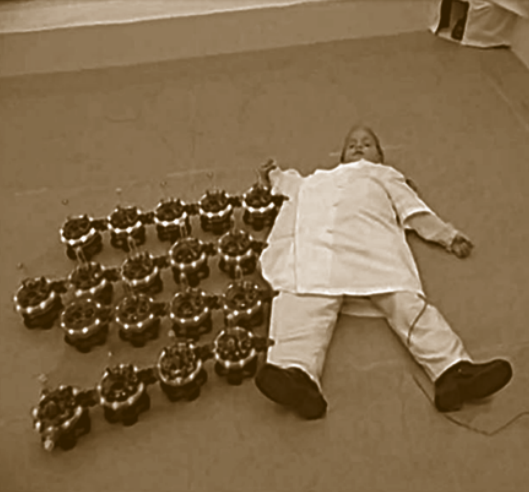
\includegraphics[scale=0.6]{figures/images/literature/child_dragged_robots.png}
    \caption{Rövid szöveg a képről, hivatkozás \cite{parker2016multiple}}
    \label{fig:child_dragged}
\end{figure}

\section{Cím 2}

Két ábra egymás mellett (lásd \ref{fig:insbots} ábra).

\begin{figure}[h]
    \centering
    \hfill
    \subfigure[Insbot \cite{colot2004insbot}]{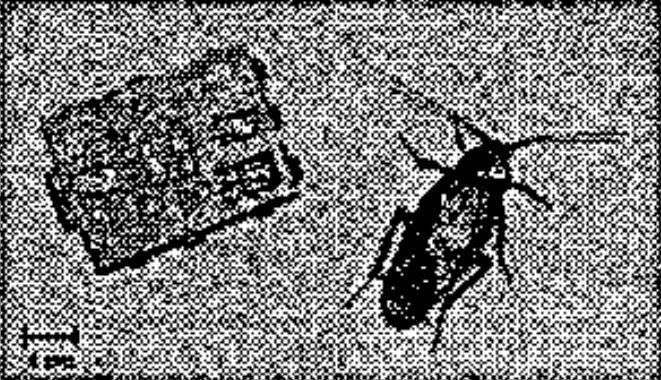
\includegraphics[scale=0.3]{figures/images/literature/insbot.png}}
    \hfill
    \subfigure[Insbot és csótányok interakciója \cite{garnier2011ants}.]{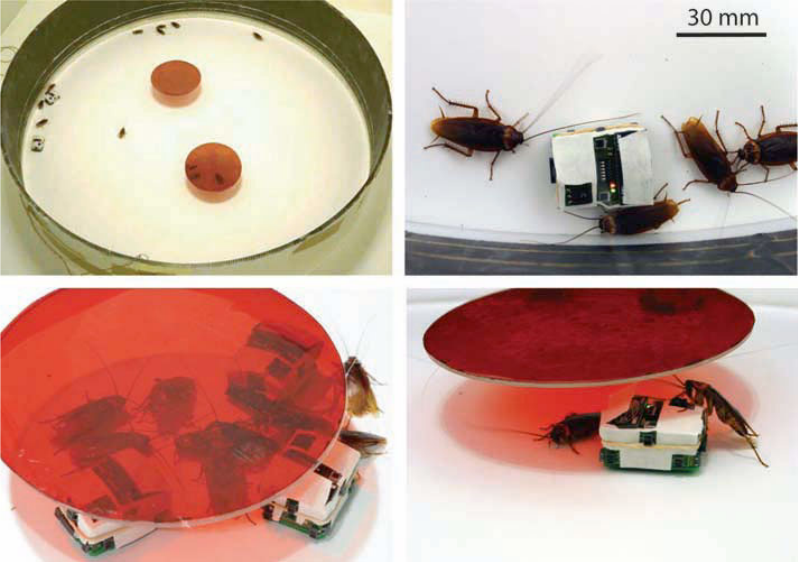
\includegraphics[scale=0.25]{figures/images/literature/insbot_cockroach.png}}
    
    \caption{Insbot és csótányok interakciója. Az insbot-ok képesek a csótányokat csalogatni.}
    \label{fig:insbots}
\end{figure}